% ****** Start of file apssamp.tex ******
%
%   This file is part of the APS files in the REVTeX 4.1 distribution.
%   Version 4.1r of REVTeX, August 2010
%
%   Copyright (c) 2009, 2010 The American Physical Society.
%
%   See the REVTeX 4 README file for restrictions and more information.
%
% TeX'ing this file requires that you have AMS-LaTeX 2.0 installed
% as well as the rest of the prerequisites for REVTeX 4.1
%
% See the REVTeX 4 README file
% It also requires running BibTeX. The commands are as follows:
%
%  1)  latex apssamp.tex
%  2)  bibtex apssamp
%  3)  latex apssamp.tex
%  4)  latex apssamp.tex
%
\documentclass[%
 reprint,
%superscriptaddress,
%groupedaddress,
%unsortedaddress,
%runinaddress,
%frontmatterverbose, 
%preprint,
%showpacs,preprintnumbers,
%nofootinbib,
%nobibnotes,
%bibnotes,
 amsmath,amssymb,
 aps,
%pra,
%prb,
%rmp,
%prstab,
%prstper,
%floatfix,
]{revtex4-1}

\usepackage{graphicx}% Include figure files
\usepackage{dcolumn}% Align table columns on decimal point
\usepackage{bm}% bold math
%\usepackage{hyperref}% add hypertext capabilities
%\usepackage[mathlines]{lineno}% Enable numbering of text and display math
%\linenumbers\relax % Commence numbering lines

%\usepackage[showframe,%Uncomment any one of the following lines to test 
%%scale=0.7, marginratio={1:1, 2:3}, ignoreall,% default settings
%%text={7in,10in},centering,
%%margin=1.5in,
%%total={6.5in,8.75in}, top=1.2in, left=0.9in, includefoot,
%%height=10in,a5paper,hmargin={3cm,0.8in},
%]{geometry}

\begin{document}

%\preprint{APS/123-QED}

\title{Assignment 1}
\author{Nicholas William Smith}
\author{Keegan H Walkup}
\author{Hong Yao}

\affiliation{
 Department of Physics, Virginia Tech, Blacksburg, VA 24060, USA% with \\
}%




\date{\today}% It is always \today, today,
             %  but any date may be explicitly specified



\maketitle

%\tableofcontents


\section{\label{sec:level1}Shortest Path on the Cone}
In this section, we discuss the shortest path from point $(x_0,y_0,z_0)$ to point $(x_1,y_1,z_1)$ on the cone 
\begin{equation}
    z=-\sqrt{x^2+y^2}
\end{equation}
in 3 dimensional space. We will use Euler-lagrange Equation to find the minimal length path and then solve the equation and get the final path function.

\subsection{\label{sec:level2}The length function on the cone}
Using cylindrical coordinates because the problem is rotationally symmetric, we have
\begin{equation}
\begin{aligned}
x&=r\cos{\theta}
\\y&=r\sin{\theta}
\\z&=z
\end{aligned}
\end{equation}
In cylindrical coordinates, the function of the cone becomes
\begin{equation}
    z=-r.
\end{equation}
For an arbitrary curve in a 3 dimensional space in a cylindrical coordinate, we have the length $l$
\begin{equation}
    l=\int ds=\int\sqrt{dr^2+r^2d\theta^2+dz^2}.
\end{equation}
Since the path should be located on the cone, we use the equation of the cone (3) in the equation for curve length (4), to get
\begin{equation}
    l=\int\sqrt{2dr^2+r^2d\theta^2}.
\end{equation}
By factorizing d$\theta$, we have
\begin{equation}
    ds=\int\sqrt{2r'^2+r^2}d\theta
\end{equation}
where $r'$ means $\frac{dr}{d\theta}$.

\subsection{\label{sec:level2}Find the function of the path}
We set
\begin{equation}
    f(r,r',\theta)=\sqrt{2r'^2+r^2}.
\end{equation}
We will find the minimum path length of this function using the Euler-Lagrange Equation
\begin{equation}
\frac{d}{d\theta}\frac{\partial f}{\partial r'}=\frac{\partial f}{\partial r}
\end{equation}
Where,
\begin{equation}
\begin{aligned}
\frac{\partial f}{\partial r}&=\frac{r}{\sqrt{2r'^2+r^2}}
\\\frac{d}{d\theta}\frac{\partial f}{\partial r'}&=\frac{2r''}{\sqrt{2r'^2+r^2}}-\frac{2r'(2r'r''+rr')}{(\sqrt{2r'^2+r^2})^3}
\end{aligned}.
\end{equation}
So,
\begin{equation}
    \frac{r}{\sqrt{2r'^2+r^2}}=\frac{2r''}{\sqrt{2r'^2+r^2}}-\frac{2r'(2r'r''+rr')}{(\sqrt{2r'^2+r^2})^3}.
\end{equation}
After simplifying, the final form of the equation is
\begin{equation}
    r^2+4r'^2-2r''r=0.
\end{equation}

We can find the solution of Eq.(11) has the following form
\begin{equation}
    r=C_1\sec{(\frac{\theta}{\sqrt{2}}+C_2)},
\end{equation}
where $C_1$ and $C_2$ are the integral constants. These constants can be fixed by considering two ends of the path.

We set
\begin{equation}
\begin{aligned}
    r_i&=\sqrt{x_i^2+y_i^2}\\
    \theta_i&=\arctan{\frac{y_i}{x_i}}
    \\z_i&=z_i
\end{aligned}\qquad i=0,1
\end{equation}
Then, we will have the following 2 equations
\begin{equation}
\begin{aligned}
r_0=C_1sec{(\frac{\theta_0}{\sqrt{2}}+C_2)}
\\r_1=C_1sec{(\frac{\theta_1}{\sqrt{2}}+C_2)}
\end{aligned}
\end{equation}
\paragraph{}When we have
\begin{equation}
    (r_0,\theta_0)\neq(r_1,\theta_1),
\end{equation}
we can get the solution of $C_1$ and $C_2$ by solving Eq.(14). The result is
\begin{equation}
\begin{aligned}
C_1&=\frac{r_0-r_1}{\sec{(\theta_0/\sqrt{2}+C_2)}-\sec{(\theta_1/\sqrt{2}+C_2)}}\\
C_2&=\arctan{\frac{r_0\cos{\theta_0/\sqrt{2}}-r_1\cos{\theta_1/\sqrt{2}}}{r_0\sin{\theta_0/\sqrt{2}}-r_1\sin{\theta_1/\sqrt{2}}}}
\end{aligned}
\end{equation}
\paragraph{} However, when we have $\theta_0=\theta_1$ or $r_0=r_1$, we cannot find a answer from Eq.(14). But it is easy to figure them out by simple analysis.
\begin{enumerate}
    \item $\theta_0=\theta_1$ means the initial point and the final point lie on the same generatrix of the cone. So the shortest path should be the generatrix which passes these two point
    \begin{equation}
        \theta=\theta_0
    \end{equation}
    \item When $r_0=r_1$, the initial and the final points lie on the same circle around the cone. And the shortest path should be the shorter part of the circle from point 1 to point 2.
\end{enumerate}

\section{A barrel in a barrel}
In this section, we will discuss the motion of a little barrel inside a larger barrel under the assumption that the little one will rotate without slipping. We give the Lagrangian of the system and then derive the equation of motion. We give an analytical result for some oscillations and also show the numerical results of general situations.
\begin{figure}[h!]
\centering
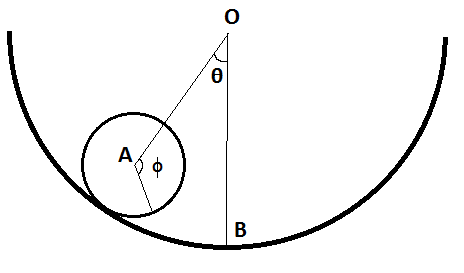
\includegraphics[scale=0.5]{Barrelception.png}
\caption{The Motion of a Barrel}
\label{fig1}
\end{figure}
\subsection{Lagrangian of the system}
In the system of a barrel rotating in another barrel in Fig.(1), there are two degree of freedom. We set $\theta$ as the angle between $\overline{OA}$ and $\overline{OB}$, where $O$ is the center of the large barrel, $A$ is the center of mass of the little barrel and $B$ is the bottom of the little barrel. And we also set $\phi$ as the rotational angle of the small barrel about its center of mass.

Thus, for the little barrel, we have its kinetic energy $T$
\begin{equation}
    T=T_{CM}+T_{Rot}
\end{equation}
where $T_{CM}$ is the kinetic energy of the center of mass and $T_{Rot}$ is the rotational kinetic energy of the little barrel about its center of mass. We have
\begin{equation}
\begin{aligned}
T_{CM}&=\frac{1}{2}M[(b-a)\dot{\theta}]^2\\
T_{Rot}&=\frac{1}{2}I\dot{\phi}^2
\end{aligned}
\end{equation}
where $I=\frac{1}{2}Ma^2$ is the moment of inertia of the little barrel among its center of mass.

For the potential energy, it will be easiest for us to set the height of point $O$ as the zero potential energy level. And then, we have
\begin{equation}
    V=-Mg(b-a)\cos{\theta}
\end{equation}
So the Lagrangian is 
\begin{equation}
\begin{aligned}
    L&=T-V\\
    &=\frac{1}{2}M(b-a)^2\dot{\theta}^2+\frac{1}{2}I\dot{\phi}^2+Mg(b-a)\cos{\theta}
\end{aligned}
\end{equation}

However, we still have one constraint on this system that the little barrel rotates without slipping. From this constraint, we can easily have 
\begin{equation}
    a\phi=b\theta.
\end{equation}

By taking Eq.(22) into Eq.(21), we have the final form of the Lagrangian
\begin{equation}
    L=\frac{1}{2}[M(b-a)^2+Mb^2]\dot{\theta}^2+Mg(b-a)\cos{\theta}
\end{equation}

\subsection{Equation of the Motion}
For the system, the Euler-Lagrange Equation is
\begin{equation}
    \frac{d}{dt}\frac{\partial L}{\partial \dot{\theta}}-\frac{\partial L}{\partial \theta}=0.
\end{equation}

Since we have
\begin{equation}
\begin{aligned}
\frac{\partial L}{\partial\dot{\theta}}=[M(b-a)^2+Mb^2]\dot{\theta}
\\\frac{\partial L}{\partial\theta}=-Mg(b-a)\sin{\theta}
\end{aligned},
\end{equation}
we obtain the equation of motion
\begin{equation}
  \ddot{\theta}+\frac{g(b-a)}{(b-a)^2+\frac{b^2}{2}}\sin{\theta}=0.
\end{equation}


\subsection{Small Oscillations}
For small oscillations, we have $\theta\rightarrow0$. So, in Eq.(26), $\sin{\theta}\rightarrow\theta$. We have
\begin{equation}
    \ddot{\theta}+\omega^2\theta=0,
\end{equation}
where $\omega^2=\frac{g(b-a)}{(b-a)^2+\frac{b^2}{2}}$.

The general solution  for Eq.(27) is 
\begin{equation}
    \theta=\theta_0\sin{(\omega t+\phi_0)},
\end{equation}
where $\theta_0$ is the amplitude of the oscillation and $\phi_0$ is the initial phase.

\begin{figure}[h!]
	\centering
	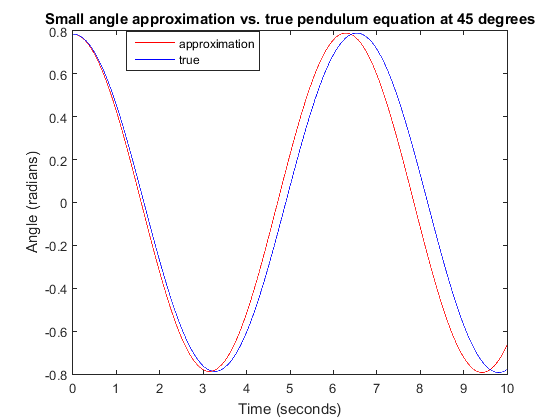
\includegraphics[scale=0.5]{Pendulum-trueVSest.png}
	\caption{Numerical Solutions}
	\label{fig2}
\end{figure}

\subsection{General Situations}
We treat the problem numerically to solve for arbitrary amplitudes using forward Euler's method.
The approximation equations we use are,
\begin{equation}
\begin{aligned}
	\theta_{i+1}& = \theta_{i} + \delta t \theta_{i}\\
	\dot{\theta}_{i+1}& = \dot{\theta_{i}} + \delta t \ddot{\theta}_{i}\\
	\ddot{\theta}_{i+1}& = - \omega^2 \theta_{i}
\end{aligned}
\end{equation}
Taking $\omega = 1$ since the mathematical form of the problem is still the pendulum despite the extra rotational energy term.
Solving gives us, We see that the small angle approximation has a period of $2\pi$ as is predicted by Eq.(29) and that the true solution has a longer period. This is expected since the next most significant term in the Taylor expansion of $sin(\theta)$ is $-\frac{x^3}{6}$, which is negative meaning a smaller acceleration. 
\begin{figure}[h!]
	\centering
	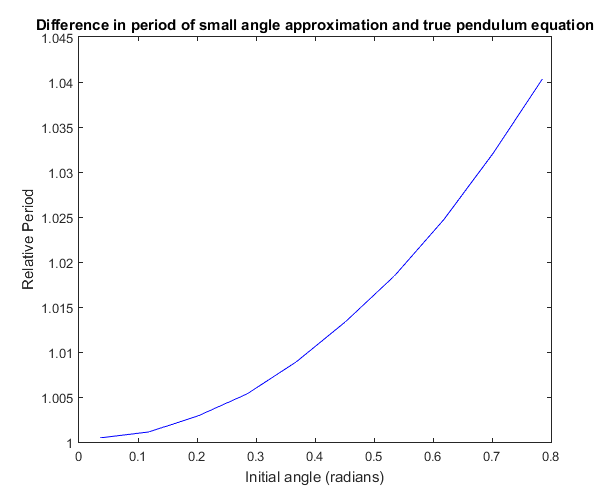
\includegraphics[scale=0.5]{Pendulum-relativeperiod.png}
	\caption{Relative Period}
	\label{fig3}
\end{figure}

We can see the general trend towards increasing period as angle increases as a percent difference. The roughly four percent difference at $45^o$ would cause a clock to be an hour slow per day.






\end{document}
%
% ****** End of file apssamp.tex ******
